\documentclass[final,hyperref={pdfpagelabels=false},xcolor=dvipsnames]{beamer}
\usepackage{grffile}
\mode<presentation>{\usetheme{Inria2}}
\usepackage[english]{babel}
%\usepackage[latin1]{inputenc}
%\usepackage{amsmath,amsthm, amssymb, latexsym}
\usepackage{tikz}
%\boldmath
\usepackage[orientation=portrait,size=a0,scale=1.4,debug]{beamerposter}
% change list indention level
% \setdefaultleftmargin{3em}{}{}{}{}{}


%\usepackage{snapshot} % will write a .dep file with all dependencies, allows for easy bundling

\usepackage{array,booktabs,tabularx}
\newcolumntype{Z}{>{\centering\arraybackslash}X} % centered tabularx columns
\newcommand{\pphantom}{\textcolor{ta3aluminium}} % phantom introduces a vertical space in p formatted table columns??!!

%\usepackage{amsmath,amssymb,amsfonts,stmaryrd}
\usepackage{graphicx}
%\usepackage[usenames,dvipsnames]{color}
\usepackage{tikz}
\usepackage{hyperref}
\usepackage[T1]{fontenc}
\usepackage{multicol}
\usepackage{booktabs}
\usepackage{subfig}
\usepackage{listings}
\lstset{%
   basicstyle=\ttfamily, %\scriptsize\ttfamily,
%   frame=single,
   breaklines=true,
}

\usepackage{float}
\floatstyle{boxed}
\newfloat{listfig}{htb}{lstfig}
\floatname{listfig}{Listing}

\floatstyle{ruled}
\newfloat{algorithm}{htbb}{algfig}
\floatname{algorithm}{Algorithm}

\listfiles

%%%%%%%%%%%%%%%%%%%%%%%%%%%%%%%%%%%%%%%%%%%%%%%%%%%%%%%%%%%%%%%%%%%%%%%%%%%%%%%%%%%%%%
\graphicspath{{figures/}}
\title{Probably Approximately Correct Learning of\\ Thomas Regulatory Networks from Time-Series Data}
%\begin{minipage}[T]{.49\textwidth}
\author{Arthur Carcano, Fran\c{c}ois Fages, Sylvain Soliman}
\institute[Inria, Universit\'e Paris Saclay]{EP Lifeware, Inria, Universit\'e Paris Saclay, France}

%%%%%%%%%%%%%%%%%%%%%%%%%%%%%%%%%%%%%%%%%%%%%%%%%%%%%%%%%%%%%%%%%%%%%%%%%%%%%%%%%%%%%%
\newlength{\columnheight}
\setlength{\columnheight}{105cm}


%%%%%%%%%%%%%%%%%%%%%%%%%%%%%%%%%%%%%%%%%%%%%%%%%%%%%%%%%%%%%%%%%%%%%%%%%%%%%%%%%%%%%%
\begin{document}
\begin{frame}[fragile]
  \begin{columns}
    % ---------------------------------------------------------%
    % Set up a column 
    \begin{column}{.49\textwidth}
      \begin{beamercolorbox}[center,wd=\textwidth]{postercolumn}
        \begin{minipage}[T]{.95\textwidth}  % tweaks the width, makes a new \textwidth
          \parbox[t][\columnheight]{\textwidth}{ % must be some better way to set the the height, width and textwidth simultaneously
            % Since all columns are the same length, it is all nice and tidy.  You have to get the height empirically
            % ---------------------------------------------------------%
            % fill each column with content            
            \begin{block}{Introduction}
              \begin{itemize}
              \item Automating the process of model building from experimental data 
is a very desirable goal to palliate the lack of modellers for many applications.
\item Despite the spectacular progress of machine learning techniques in data analytics, classification, clustering and prediction making,
learning dynamical models from data time-series is still challenging.
\item In this paper \cite{CFS17cmsb} we investigate the use of the Probably Approximately Correct (PAC) learning 
framework of Leslie Valiant \cite{Valiant84cacm} as a method for the automated discovery of influence models of biochemical processes from Boolean and stochastic traces. 
\item We evaluate the performance of this approach on a model of T-lymphocyte
differentiation \cite{RRMTC06tcsb,Mendoza06biosystems}, with and without prior knowledge,
and discuss its merits as well as its limitations with respect to realistic experiments.
              \end{itemize}              
            \end{block}
            \vfill
            \begin{block}{PAC Learning Protocol}
The idea behind the PAC learning protocol is to discover a Boolean
function, $G$, which approximates a hidden function $F$, while restricting oneself to the two following operations:
\begin{itemize}
  \item
{\bf Sample}$()$: returns a positive example, i.e.~a vector $v$ such that $F(v)=1$.
The output of {\bf Sample}$()$ is assumed to follow a given probability distribution $D(v)$, which is used to measure the approximation of the result.
  \item
{\bf Oracle}$(v)$: returns the value of $F(v)$ for any input vector $v$.
\end{itemize}
            \end{block}
            \vfill
            \begin{block}{Learnable Boolean Functions \cite{Valiant84cacm}}
%\begin{definition}[\cite{Valiant84cacm}]\label{def:learnclass}
   A class $\cal M$ of \emph{Boolean functions} is said to be {\bf learnable}
   if there exists an algorithm $\cal A$ with some {\bf precision parameter $h\in\mathbb N$} such that:
   \begin{itemize}
      \item $\cal A$ runs in polynomial time both in $n$ and $h$;
      \item
         for any function $F$ in $\cal M$, and any distribution $D$ on the positive examples,
         $\cal A$ deduces with {\bf probability higher than $1-h^{-1}$} an approximation $G$ of $F$ such that
         \begin{itemize}
            \item $G(v)=1$ implies $F(v)=1$ ({\bf no false positive})
            \item
               $\displaystyle\sum_{v\ s.t.\ F(v)=1\wedge G(v)=0} D(v) < h^{-1}$ ({\bf few false negatives})
         \end{itemize}
   \end{itemize}
%\end{definition}
            \end{block}
            \vfill
            \begin{block}{PAC Learning Algorithms \cite{Valiant84cacm}}
\begin{itemize}
\item
%\begin{theorem}[\cite{Valiant84cacm}]\label{thm:kcnf}
For any $k$, the class of {\bf $k$-CNF formulae} on $n$ variables is learnable with an
algorithm that uses $L(h,S)\small\le 2h(S+\log_e h)$ positive examples and no call to the
oracle, where $S=2n^{k+1}$.
%\end{theorem}
%\begin{algorithm}
\begin{enumerate}
  \item initialise $g$ to the conjunction of all the $(2n)^k$ possible clauses of at most $k$ literals,
\item do $L(h,(2n)^{k+1})$ times 
\begin{enumerate}
\item $v:=\textsc{Sample}()$
\item delete all the clauses in $g$ that do not contain a literal true in $v$
\end{enumerate}
\item output: $g$
\end{enumerate}
%\caption{PAC-learning of $k$-CNF formulae.\label{algCNF}}
%\end{algorithm}
%\begin{theorem}[\cite{Valiant84cacm}]\label{thm:mdnf}
\item
    The class of {\bf monotone DNF formulae} on $n$ variables is also learnable with an
    algorithm that uses $L(h,d)$ examples and $d n$ calls to the oracle,
    where $d$ is the largest number of prime implicants of the function to learn.
%\end{theorem}
\end{itemize}
            \end{block}
            \vfill
            \begin{block}{T-helper Lymphocyte Differentiation Inlfuence Graph \cite{RRMTC06tcsb}}
   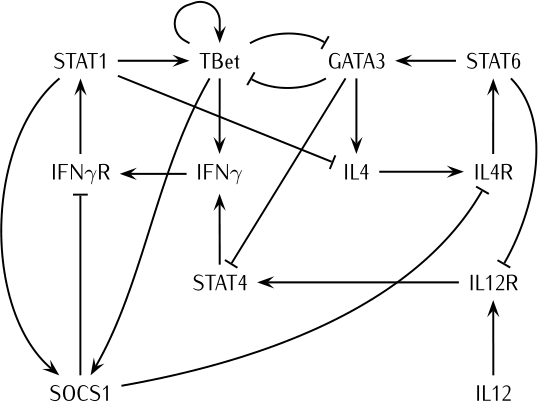
\includegraphics[width=0.8\textwidth]{th_net_clean.png}
	    \end{block}
            \vfill
          }
        \end{minipage}
      \end{beamercolorbox}
    \end{column}
    % ---------------------------------------------------------%
    % end the column
    
    % ---------------------------------------------------------%
    % Set up a column 
    \begin{column}{.49\textwidth}
      \begin{beamercolorbox}[center,wd=\textwidth]{postercolumn}
        \begin{minipage}[T]{.95\textwidth} % tweaks the width, makes a new \textwidth
          \parbox[t][\columnheight]{\textwidth}{ % must be some better way to set the the height, width and textwidth simultaneously
            % Since all columns are the same length, it is all nice and tidy.  You have to get the height empirically
            % ---------------------------------------------------------%
            % fill each column with content
            \begin{block}{Influence System in BIOCHAM v4 syntax (DNF form)}
%\begin{listfig}[htb]
\footnotesize
   \lstinputlisting[multicols=2,firstline=6]{examples/lympho.bc}
%\end{listfig}
	    \end{block}
            \vfill
            \begin{block}{Results of PAC Learning from Stochastic Simulation Traces}
\begin{itemize}
\item
{\bf Space-time tradeoff}: many short traces better than few long traces

%\begin{figure}[htb]
  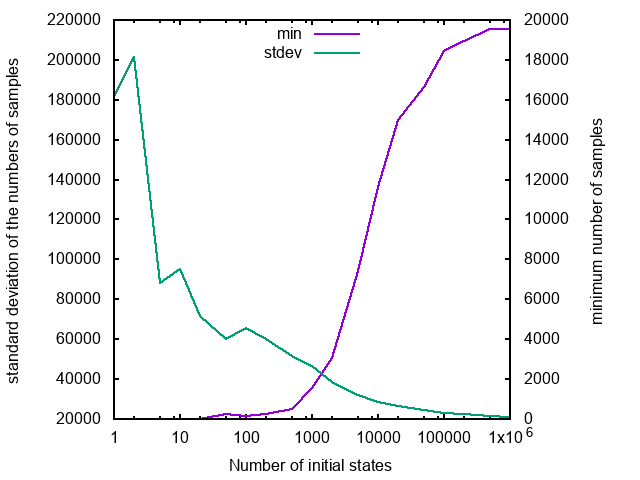
\includegraphics[width=0.9\textwidth]{statistics/statistics.png}
   %\caption{
\begin{itemize}
\item
Minimum number of (de)activation samples,
\item Standard deviation
\item {\bf Model error} (number of false positives and false negatives) 
\end{itemize}
obtained for the 24 boolean functions of the Th-lymphocyte example, 

as a function of the number of initial states 

(with total number of samples kept constant by adjusting the time horizon). %}
%\label{fig:statistics}
%\end{figure}
\item
{\bf Correct model learned from 500 traces}: below, some rare transitions are not observed resulting in the building of complex models.
\item
Giving the influence graph as prior knowledge reduces the number of possible clauses $S<<(2n)^{k+1}$ in \(samples = 2h(S + \log h)\).
%Learn correct model from ???? traces.
\end{itemize}
	    \end{block}
            \vfill
  	    \begin{block}{Conclusions}
              \begin{itemize}
              \item Valiant's work on PAC learning provides an elegant trail, with {\bf error bounds},
to attack the challenge of inferring the structure of influence models from the observation of data time series,
%and more precisely to automatically discover possible regulatory networks of a biochemical process, given sufficiently precise observations of its executions.
\item The Boolean dynamics of biochemical influence systems, including Thomas regulatory networks, can be represented by $k$-CNF formulae without loss of generality,
and $k$-CNF PAC learning algorithm can be used to infer the structure of the network,
and bound the errors made according to the {\bf distribution of the state transition samples}. 
\item {\bf Many short traces better than few long traces} in line with the pratice of integrative analyses
such as~\cite{CCCCNT04mbc} and its more than 130 mutants.
              \end{itemize}
\footnotesize


\bibliographystyle{splncs03}
\bibliography{contraintes}

\vfill
            \end{block}
            \vfill
          }
          % ---------------------------------------------------------%
          % end the column
        \end{minipage}
      \end{beamercolorbox}
    \end{column}
    % ---------------------------------------------------------%
    % end the column
  \end{columns}
  \vskip1ex
  %\tiny\hfill\textcolor{ta2gray}{Created with \LaTeX \texttt{beamerposter}  \url{http://www-i6.informatik.rwth-aachen.de/~dreuw/latexbeamerposter.php}}
  %\tiny\hfill{Created with \LaTeX \texttt{beamerposter}  \url{http://www-i6.informatik.rwth-aachen.de/~dreuw/latexbeamerposter.php} \hskip1em}
\end{frame}
\end{document}


%%%%%%%%%%%%%%%%%%%%%%%%%%%%%%%%%%%%%%%%%%%%%%%%%%%%%%%%%%%%%%%%%%%%%%%%%%%%%%%%%%%%%%%%%%%%%%%%%%%%
%%% Local Variables: 
%%% mode: latex
%%% TeX-PDF-mode: t
%%% End:
